%----------------------------------------------------------------------------------------
%	PACKAGES AND OTHER DOCUMENT CONFIGURATIONS
%----------------------------------------------------------------------------------------
\documentclass[paper=a4, fontsize=11pt]{scrartcl} % A4 paper and 11pt font size
\usepackage[T1]{fontenc} % Use 8-bit encoding that has 256 glyphs
\usepackage{fourier} % Use the Adobe Utopia font for the document - comment this line to return to the LaTeX default
\usepackage[english]{babel} % English language/hyphenation
\usepackage{amsmath,amsfonts,amsthm} % Math packages
\usepackage{lipsum} % Used for inserting dummy 'Lorem ipsum' text into the template
\usepackage{sectsty} % Allows customizing section commands
\allsectionsfont{\centering \normalfont\scshape} % Make all sections centered, the default font and small caps
\usepackage{fancyhdr} % Custom headers and footers
\usepackage[]{mcode}
\usepackage{amsmath}
\usepackage{graphics}
\usepackage{graphicx}

\pagestyle{fancyplain} % Makes all pages in the document conform to the custom headers and footers
\fancyhead{} % No page header - if you want one, create it in the same way as the footers below
\fancyfoot[L]{} % Empty left footer
\fancyfoot[C]{} % Empty center footer
\fancyfoot[R]{\thepage} % Page numbering for right footer
\renewcommand{\headrulewidth}{0pt} % Remove header underlines
\renewcommand{\footrulewidth}{0pt} % Remove footer underlines
\setlength{\headheight}{13.6pt} % Customize the height of the header

\numberwithin{equation}{section} % Number equations within sections (i.e. 1.1, 1.2, 2.1, 2.2 instead of 1, 2, 3, 4)
\numberwithin{figure}{section} % Number figures within sections (i.e. 1.1, 1.2, 2.1, 2.2 instead of 1, 2, 3, 4)
\numberwithin{table}{section} % Number tables within sections (i.e. 1.1, 1.2, 2.1, 2.2 instead of 1, 2, 3, 4)

\setlength\parindent{0pt} % Removes all indentation from paragraphs - comment this line for an assignment with lots of text

%----------------------------------------------------------------------------------------
%	TITLE SECTION
%----------------------------------------------------------------------------------------

\newcommand{\horrule}[1]{\rule{\linewidth}{#1}} % Create horizontal rule command with 1 argument of height

\title{	
\normalfont \normalsize 
\horrule{0.5pt} \\[0.4cm] % Thin top horizontal rule
\huge ECE 532 Homework 5:\\ % The assignment title
\horrule{2pt} \\[0.5cm] % Thick bottom horizontal rule
}

\author{Qihong Lu} % Your name
\date{\normalsize\today} % Today's date or a custom date

\begin{document}

\maketitle % Print the title

%----------------------------------------------------------------------------------------
%	PROBLEM 1
%----------------------------------------------------------------------------------------

\section*{Question1 Face recognition}

Here I am providing a high level explanation of what I did. For clarity, the cross validation procedure is not included here. I did what was requested in the instruction. \\ 

\textbf{a) Truncated SVD}\\
First, I computed the economy SVD: $X = U \Sigma V^T$. Then, to truncate the solution, I computed  $\Sigma^{-1}$, then I set the smallest n diagonal values to zero, where n is the number of rank that I want to remove. Here, we can truncate 0 to 8 singular values. In other words, we can use 1 to 9 singular values to perform the classification, and using 9 singular values corresponds to no truncation. Let me denote the truncated $\Sigma^{-1}$ by $\Sigma_t^{-1}$. 

Then the weights $\beta$ for the features were computed by: 
$$\beta = V \Sigma_t^{-1} U^T y$$

And I computed the prediction as follows: 

$$\text{predictions} = sign(X \beta)$$

Namely, in the vector $X_{test} \beta$, positive values were considered as 1, negative values were considered as -1.\\


\textbf{b) Regularized Least square}\\
This is just a standard least square procedure with a regularzation, but I computed it with SVD. Initially, to obtain the weights, $\beta$, for the features, I do the following: 
$$ \beta = (X^T X + \lambda I)^{-1} X^T y $$ 
Now, if $X = U \Sigma V^T$ (the economy SVD), then 
$$ \beta_{svd} = V (\Sigma^2 + \lambda I)^{-1} \Sigma  U^T y $$ 

I used the SVD solution to compute the $\beta_{svd}$ in the assignment. I verified that it matches with the old way of computing $\beta$ by checking ensuring all elements in $\beta_{svd}$ are equal to corresponding elements in $\beta$ (absolute value of the difference smaller than $10^{-12}$). \\



\textbf{Compare the performance of the truncated SVD and regularized least square. }\\

I compared these two methods in terms there corss-validated error on the final hold out set (n=56 for both methods). \\

When truncating SVD, if there are multiple truncations give to same cross validated best accuracy, then I pick the solution with the lowest rank (use as less information as possible). When doing regularized least square, if there are multiple parameter give the same best accuracy, then I chose the smallest parameter. When this way of choosing parameter. \\

The mean accuracy on the hold out set for truncated SVD is: 0.1116 (SD = 0.1190).\\
The mean accuracy on the hold out set for regularized LS is: 0.0480 (SD = 0.0477).\\
Moreover, t-test suggests that they are regularized LS performed better than truncated SVD (t = 4.11, p = 7.7826e-05 < 0.001, two-tailed). In this case, truncated SVD performed worse than regularized LS. \\

However, if I change my definition of the best parameter for truncated SVD, the results looked different. The new policy is that, among all truncations, pick the one with the largest rank (use as much information as possible), then the performance of the truncated SVD and regularized LS are indistinguishable. \\

So in general, the relative performance of the two methods depends on how do we define the "best parameter". \\


\textbf{c) Add new features by taking linear combinations of the original features}\\


This should be problematic. When adding three columns of X by taking linear combinations of the original columns of X, it creates dependence. Therefore, when doing the SVD: $X = U \Sigma V^T$, S would have three zero entries on the lower right. 

In the case of truncated SVD, computing $\beta$ relies on the following formula: 
$$\beta = V \Sigma_t^{-1} U^T y$$
where $\Sigma_t^{-1}$ is computed by inverting $\Sigma$ then truncate the smaller values on the diagnal. However, because some diagnoal entries would be zero, $\Sigma$ is not going to be invertible. When doing numerical computation, the smallest singular values are not going to be zero exactly, but they will be very close to zero. \\


In the case of regularized LS, we need to compute 
$$ \beta_{svd} = V (\Sigma^2 + \lambda I)^{-1} \Sigma  U^T y $$ 
but $(\Sigma^2 + \lambda I)^{-1}$ is not going to be invertible and this results might be different from the results given by the normal equation. For the same reason stated above, the three diagonal entries on the lower right of $\Sigma^2$ would be nearly zeros. And when adding $\lambda I$, where lambda is a small number, the three diagonal entries on the lower right would be very small, and inverting it would make them very large. So the results would be more variable. \\ 


To check my idea, I did some simulation. I ran classification with 3 additional features 10 times. Because the 3 additional features involve randomness so the results can vary. I also ran the classification without additional feature, and there is no randomness here. Then I compare their performance by doing t test. \\

The statistical results indicate that both svd and ridge classifer performed worse when adding additional 3 features (both P < 0.05), compared to the classifer without those three redundent features. Matlab also reported that the matrices are almost singular. \\

(When I did this comparison, the best rank for the truncated SVD was chosen by using the largest rank if multiple rank are equally good at classification performance)

Here's the code for the statistical testing: 
\begin{lstlisting}
clear all; close all; clc; 
% compute the performance for ridge and svd, set this as the baseline
[baseLineAcc] = faceRecog(0);
% compute the performance for ridge and svd when adding 3 redundent features 
sampSize = 10;
accuracy = cell(sampSize,1);
for i = 1 : sampSize
    accuracy{i} = faceRecog(1);
end
meanAcc.svd = []; meanAcc.ridge = [];
for i = 1 : sampSize
    meanAcc.svd = [meanAcc.svd mean(accuracy{i}.svd(:))];
    meanAcc.ridge = [meanAcc.ridge mean(accuracy{i}.ridge(:))];
end

% t test, see if their difference is zero 
[h1,p1,ci1,stats1] = ttest(meanAcc.svd - mean(baseLineAcc.svd(:)))
[h2,p2,ci2,stats2] = ttest(meanAcc.ridge - mean(baseLineAcc.ridge(:)))

\end{lstlisting}

\newpage
Here's the code for the classifer 
\begin{lstlisting}
function [finalAcc] = faceRecog(addNewFeatures)
%% load data
load('face_emotion_data.mat')

%% add new features: random linear combinations of original features
% addNewFeatures = 1;
if addNewFeatures
    % create 3 new features as random linear combinations of original features
    newFeatures = X * randn(size(X,2),3);
    X = [X newFeatures];
end


%% set parameters
[m,n] = size(X);
CVBSize = 16;       % cross validation block size (diviside by m)
maxRank = n;
LAMBDAS = [0 2.^(-1 : 4)];  % L2 reg. parameters that we want to try
I = eye(n);

%% set up the final hold-out set
[finalHoldoutIdx, K_full] = setupCVBlocks(size(X,1), CVBSize);

% loop over all possible final hold out set (8 of them)
for k = 1 : K_full;
    % hold out 1 chunk as the final test set
    X_part = X(~finalHoldoutIdx(:,k),:);
    y_part = y(~finalHoldoutIdx(:,k));
    X_final = X(finalHoldoutIdx(:,k),:);
    y_final = y(finalHoldoutIdx(:,k));
    
    %% setup tuning sets cross-validation blocks for the tunning procedure
    % loop over all possible tuning hold out set (7 of them)
    [holdoutIdx, K_tune] = setupCVBlocks(size(X_part,1), CVBSize);
    
    for i = 1:K_tune
        % split the data into training and test set
        X_train = X_part(~holdoutIdx(:,i),:);
        y_train = y_part(~holdoutIdx(:,i));
        X_test = X_part(holdoutIdx(:,i),:);
        y_test = y_part(holdoutIdx(:,i));
        
        testAccuracy = nan(maxRank,1);
        % compute the singular value decomposition
        [U,S,V] = svd(X_train, 'econ');
        for rank = 1:maxRank;
            %% fit the model
            S_inv_truncate = truncateS(inv(S), rank);
            % compute the beta with U,S,V
            beta_svd(:,rank) = V * S_inv_truncate * U' * y_train;
            % make the prediction
            predict = ones(CVBSize,1);
            predict(X_test * beta_svd(:,rank) <= 0) = -1;
            % evaluate the performance
            correctPred = bsxfun(@eq, predict, y_test);
            testAccuracy(rank) = sum(correctPred) / CVBSize;
        end
        
        %% test the best beta with the final hold out set
        % find the best rank
        bestRank = find(testAccuracy == max(testAccuracy) ,1, 'last');
        % generate predictions 
        predict = ones(CVBSize,1);
        predict(X_final * beta_svd(:,bestRank) <= 0) = -1;
        % evaluate the performance
        correctPred = bsxfun(@eq, predict, y_final);
        finalAcc.svd(i,k) = sum(correctPred) / CVBSize;
        
        %% fitting ridge regression 
        testAccuracy = nan(length(LAMBDAS),1);
        % compute SVD
        [U,S,V] = svd(X_train, 'econ');
        for l = 1:length(LAMBDAS)
            % choose a lambda value 
            lambda = LAMBDAS(l);
            %% fit the model
            % compute the beta with U,S,V
            beta_ridge(:,l) = V * inv(S^2 + I*lambda) * S * U' * y_train;
            % compute the beta with the normal equations
            beta_check = inv(X_train' * X_train + I*lambda) * X_train' * y_train;
            % check if they are the same
            if any(abs(beta_check - beta_ridge(:,l)) > 1e-12)
                warning('WARNING: SVD solution and normal equations solution are different!')
            end
            % make the prediction
            predict = ones(CVBSize,1);
            predict(X_test * beta_ridge(:,l) <= 0) = -1;
            % evaluate the performance
            correctPred = bsxfun(@eq, predict, y_test);
            testAccuracy(l) = sum(correctPred) / CVBSize;
        end
        
        %% check the best weights using the final hold out set
        % find the best rank
        bestLambdaIdx = find(testAccuracy == max(testAccuracy) ,1, 'first');
        % generate predictions 
        predict = ones(CVBSize,1);
        predict(X_final * beta_ridge(:,bestLambdaIdx) <= 0) = -1;
        %% evaluate the performance
        correctPred = bsxfun(@eq, predict, y_final);
        finalAcc.ridge(i,k) = sum(correctPred) / CVBSize;
        
    end % end of one tuning set 
end % end of one final hold out set

%% compare performance
mean(finalAcc.svd(:))
mean(finalAcc.ridge(:))

error.svd = 1 - finalAcc.svd;
error.ridge = 1 - finalAcc.ridge;
[H,P,CI,STATS] = ttest(error.svd(:),error.ridge(:))

end % end of definition of the main 
%%%%%%%%%%%%%%%%%%%%%%%%%%%%%%%%%%%%%%%%%%%%%%%%%%%%%%%%%%%%%%%%%%%%%%%%%%%%%
%%%%%%%%%%%%%%%%%%%%%%%% Helper functions %%%%%%%%%%%%%%%%%%%%%%%%%%%%%%%%%%%
%%%%%%%%%%%%%%%%%%%%%%%%%%%%%%%%%%%%%%%%%%%%%%%%%%%%%%%%%%%%%%%%%%%%%%%%%%%%%

%% set up the cv blocks
function [holdOutIdx, numFolds] = setupCVBlocks(numData, cvBlockSize)
numFolds = numData/cvBlockSize;
holdOutIdx = false(numData,numFolds);        % the indicies for the hold out set
% get the hold out set indices for K folds
for i = 1 : numFolds
    holdOutIdx(((i-1)*cvBlockSize+1):(i)*cvBlockSize,i) = true;
end
end

%% truncate the diagnal matrix S: leave the first r diagnal entries
function S_truncate = truncateS(S, rank)
% truncate singular values
S_truncate = S;
for i = rank+1 : length(diag(S))
    S_truncate(i,i) = 0;
end
end

\end{lstlisting}

\newpage
%----------------------------------------------------------------------------------------
%	PROBLEM 2
%----------------------------------------------------------------------------------------

\section*{Question2 Signal reconsturction}

\textbf{(a)} I implemented least square, truncated SVD, and regularized LS methods. The code is attached at the end for clarity. For the blurred signal, $k = 30, sigma = 0.01$

(i) For least square, there is no parameter. \\
(ii) For truncated SVD, since the possible parameter is too large (about 500 of them, which corresponds to the number of features in the data set), I chose the parameter to be 1, 20, 40, 60, ..., 480, 500. \\
(iii) For L2 regularized least square, I chose the list of parameters to be $0, 2^{-13}, 2^{-12}, 2^{-11}, ... 2^{10}, 2^{11}$\\ 

Let y be the predicted value (blurred signal), and $\beta$ be the weights assigned for each feature (true signal). For each parameter, I fitted a model and computed its predicted blurred signal (y) and true signal (beta). 
\begin{center}
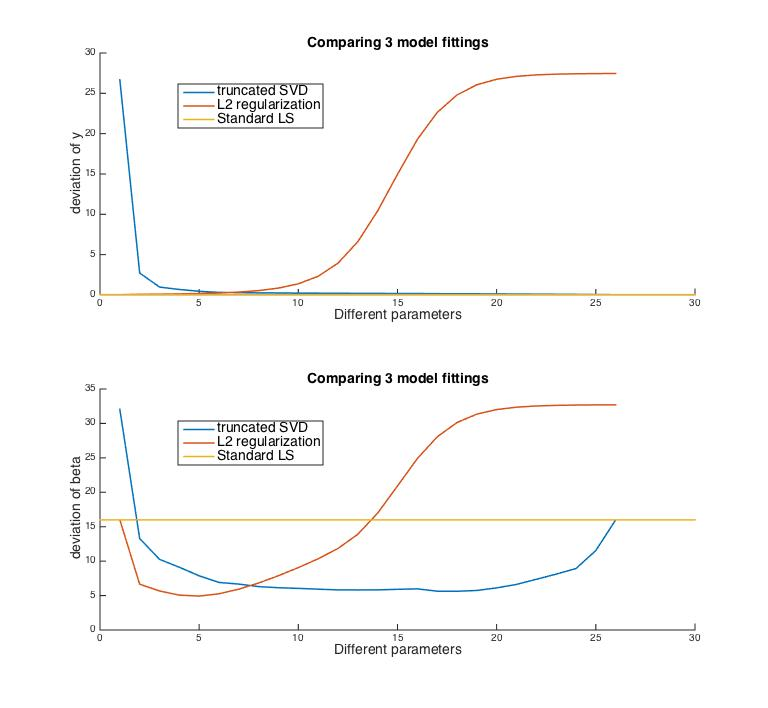
\includegraphics[scale=.5]{2a_compare3models.jpg}
\end{center}
The plot on the top is showing the deviation of the predicted y and ture y, for all parameter I tried. The plot at the buttom is showing the analog for beta. Since standard least square method has no parameter, its performance is flat. 

The plot on the top shows that all 3 models performed pretty well at fitting blurred signal, y. The standard least square has very low deviation on y. Also, with appropriate parameter choice, both truncated SVD and ridge regression can achieve very small deviation on y. \\

However, the plot on the buttom shows that the standard least square failed to fit the true signal, beta. In comparison, both truncated SVD and ridge regression can fit the true signal pretty well, with appropriate parameter. \\\\

To visualize the how well "the best parameter" fit with the true signal, I found "the best beta" for truncated SVD and regularized least square and plotted their fits below. Here, the best beta is defined as being the best at minimizing the 2 norm of predicted beta versus true beta. 

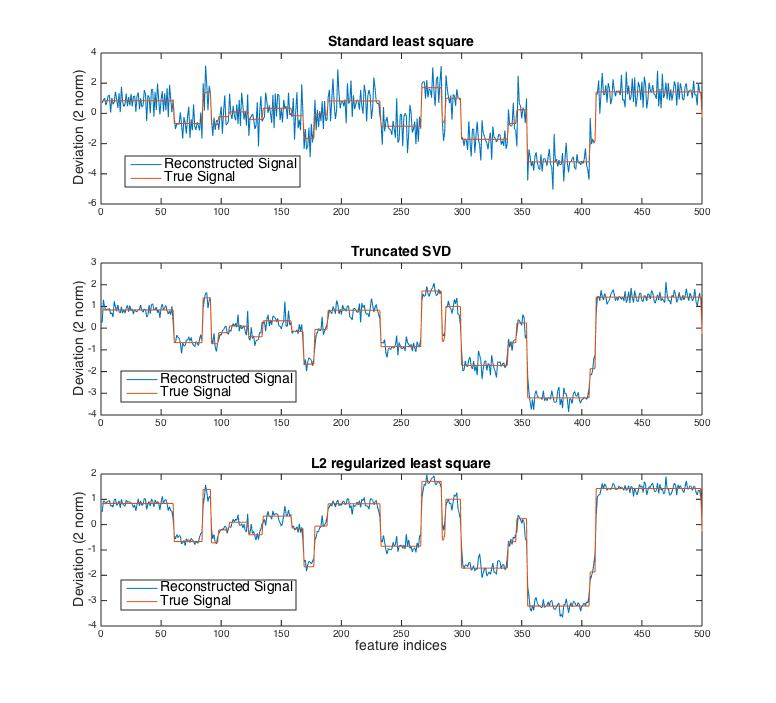
\includegraphics[scale=.5]{2a_compareBetas.jpg}

From these plots, we can confirm that both truncated SVD and regularized least sqaure can fit the data pretty well, whereas the standard least square performed qualitatively worse than the two alternatives. 

\newpage
\textbf{b) How blurring and noise level affect the value of regularization parameter that produce the best estimates?}\\

Since reconstruct the true signal beta is more important, I ignored the data for fitting the blurred signal, y, and focus on the true signal, beta, in this discussion. \\

\textit{1. Varying noise while fixing k}
\begin{center}
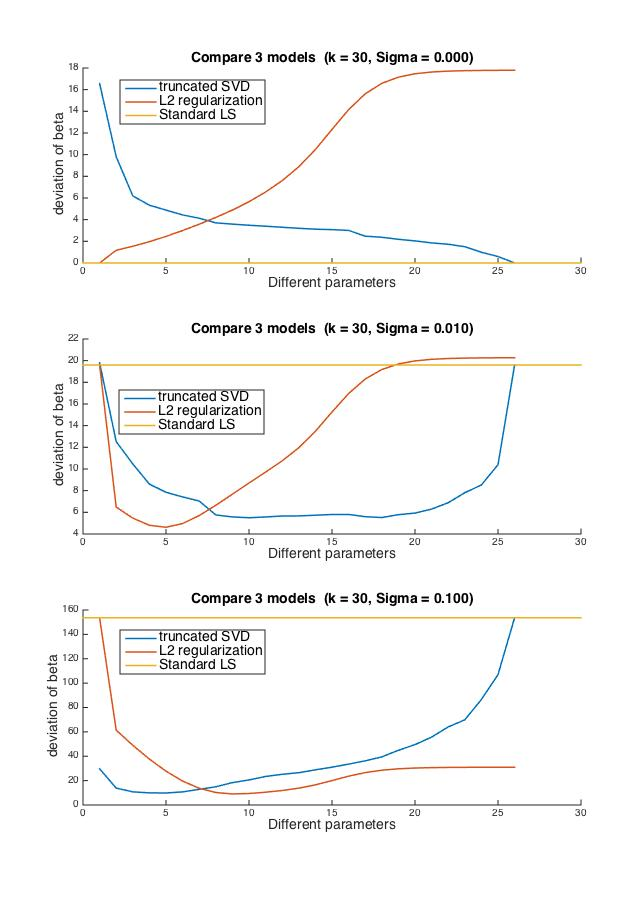
\includegraphics[scale=.54]{2b_varyNoise.jpg}
\end{center}

From top to buttom, I am fixing k (= 30) while increasing the noise level: 0, 0.1 and 0.01. The optimal performance for truncated SVD and ridge regression is represented by their minimums. \\ 

When increasing noise, the truncated SVD "perfers" to use less ranks. This is because when the noise is big, it is harder to tell if principle compoenents with small singular values are capturing noise or true signal. In contrast, when the noise is small, using principle components with small singular values is still relatively safe. \\

For the regularized least square solution, The minimum is shifting towards the right when increasing the noise. When there is no noise, no regularization is needed to achieve the smallest deviation. When there are more noises, more regularization is needed. This make sense, when there is no noise, regularizing features is going to bias the results. However, when there are a lot of noises, some features might be altered by the noise too much, so using them would leads to bad estimation. Therefore, higher regularzation parameter would force the classifer to minimize the weights associated with all features, which in turn, minimized the weights for the noise.  \\

For the standard least square, there is no parameter. Its performance is simply getting better when there is less noise, which make sense. 

\newpage
\textit{2. Varying k while fixing noise}
\begin{center}
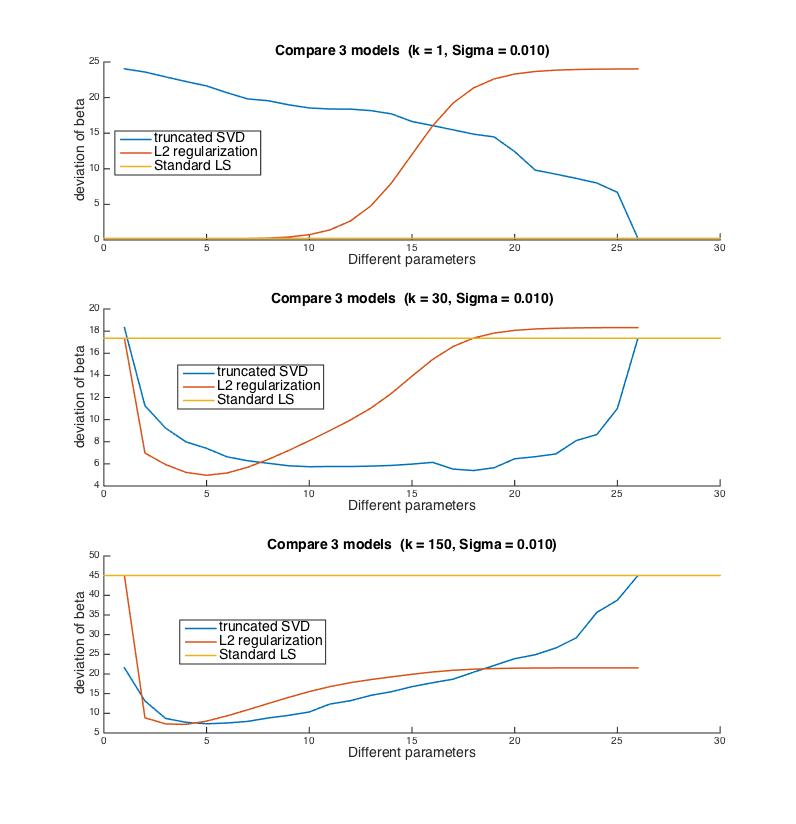
\includegraphics[scale=.6]{2b_varyk.jpg}
\end{center}

Not I am fixing the noise level 0.01, while varying k: 1, 30, 150. Here, k is a spatial blurring factor. When k is large, the signal is more spreaded out to the neighbouring locations. \\

When increase the spatial bluring factor k, the truncated SVD "perfers" smaller rank. Because having more principle components might captures misleading information. In particular, when there is no spatial blurring, the truncated SVD picked up almost all principle components (the top plot), and when there is a large spatial blurring, using less ranks had better fit to the true signal (the buttom plot). \\

For regularized least square, the genearl trend is less clear. When there is no spatial blurring, no regularization is needed to achieve the closest fit (the top plot). This is because regularizing the weights for the features without any blurring is going to make them less accurate. When there is more spatial blurring (the middle plot), it is good to do regularize the weights slightly. When the spatial blurring is huge (the buttom plot), using big lambda versus intermediate lambda made little difference.\\

Again, when increasing the spatial blurring, the least square performance decreases monotonically. 

\newpage
\begin{lstlisting}
%% signal reconstruction
function blurData3()
% load the data
k = 30; 
sigma = 0.1; 
[X, y, btrue] = generateBluringData(k,sigma);
%% set the choice of parameter 
LAMBDAS = [0 2.^(-13 : 11)];
RANK = [1 20:20:500];
normType = 2; 

%% standard LS
beta.ls = inv(X' * X) * X' * y;
% make the prediction
deviation.ls = y - X * beta.ls;
% save 1 norm of deviation (parameter by CV block)
deviationY_1norm.ls = norm(deviation.ls,normType);
deviationB_1norm.ls = norm(beta.ls - btrue,normType);

%% truncated SVD
[U,S,V] = svd(X, 'econ');
for p = 1:length(RANK);
    rank = RANK(p);
    % fit the model
    S_inv_truncate = truncateS(inv(S), rank);
    % compute the beta with U,S,V
    beta.svd(:,p) = V * S_inv_truncate * U' * y;
    % make the prediction
    deviation.svd = y - X * beta.svd(:,p);
    % save 1 norm of deviation (parameter by CV block)
    deviationY_1norm.svd(p) = norm(deviation.svd,normType);
    deviationB_1norm.svd(p) = norm(beta.svd(:,p) - btrue, normType);
end

%% RLS
I = eye(size(S));
for l = 1:length(LAMBDAS)
    % choose a lambda value
    lambda = LAMBDAS(l);
    % compute the beta with U,S,V
    beta.ridge(:,l) = V * inv(S^2 + I*lambda) * S * U' * y;
    % make the prediction
    deviation.rid = y - X * beta.ridge(:,l);
    % save 1 norm of deviation (parameter by CV block)
    deviationY_1norm.rid(l) = norm(deviation.rid,normType);
    deviationB_1norm.rid(l) = norm(beta.ridge(:,l) - btrue, normType);
end


%% plot the performance 
close all; 
subplot(2,1,1)
plotDeviation_y(deviationY_1norm, 'deviation of y')
subplot(2,1,2)
plotDeviation_y(deviationB_1norm, 'deviation of beta')


%% visualize predicted betas against the truth
figure;
plotBetaDeviation(deviationB_1norm, beta, btrue, normType);
end

%%%%%%%%%%%%%%%%%%%%%%%%%%%%%%%%%%%%%%%%%%%%%%%%%%%%%%%%%%%%%%%%%%%%%%%%%%%%%
%%%%%%%%%%%%%%%%%%%%%%%% Helper functions %%%%%%%%%%%%%%%%%%%%%%%%%%%%%%%%%%%
%%%%%%%%%%%%%%%%%%%%%%%%%%%%%%%%%%%%%%%%%%%%%%%%%%%%%%%%%%%%%%%%%%%%%%%%%%%%%

%% plot predicted beta against truth
function plotBetaDeviation(deviation, beta, btrue, normType)
FS = 14;
ylab_text = sprintf('Deviation (%d norm)', normType);
% find the index for the "best beta"
bestRidgeIdx = deviation.rid == min(deviation.rid);
bestSvdIdx = deviation.svd == min(deviation.svd);

% plot them 
subplot(3,1,1)
plot([beta.ls btrue])
legend({'Reconstructed Signal', 'True Signal'}, 'fontsize', FS, 'location', 'southeast')
title('Standard least square', 'fontsize', FS)
ylabel(ylab_text, 'fontsize', FS)
subplot(3,1,2)
plot([beta.svd(:,bestSvdIdx) btrue])
legend({'Reconstructed Signal', 'True Signal'}, 'fontsize', FS, 'location', 'southeast')
title('Truncated SVD', 'fontsize', FS)
ylabel(ylab_text, 'fontsize', FS)
subplot(3,1,3)
plot([beta.ridge(:,bestRidgeIdx) btrue])
legend({'Reconstructed Signal', 'True Signal'}, 'fontsize', FS, 'location', 'southeast')
title('L2 regularized least square', 'fontsize', FS)
ylabel(ylab_text, 'fontsize', FS)
xlabel('feature indices', 'fontsize', FS)

end

%% function: plot deviation on y
function [] = plotDeviation_y(dev1norm, ylabel_text)
LWD = 1.5;
FS = 14;
hold on
plot(dev1norm.svd, 'linewidth', LWD)
plot(dev1norm.rid, 'linewidth', LWD)
plot(xlim,[dev1norm.ls dev1norm.ls], 'linewidth', LWD)
plot(xlim,5)
hold off
legend({'truncated SVD', 'L2 regularization', 'Standard LS'}, ...
    'fontsize', 14, 'location', 'northwest')
title('Comparing 3 model fittings', 'fontsize', FS)
ylabel(ylabel_text, 'fontsize', FS)
xlabel('Different parameters', 'fontsize', FS)
end

%% truncate the diagnal matrix S: leave the first r diagnal entries
function S_truncate = truncateS(S, rank)
% truncate singular values
S_truncate = S;
for i = rank+1 : length(diag(S))
    S_truncate(i,i) = 0;
end
end
\end{lstlisting}




\end{document}